\documentclass[a4paper]{ltjsarticle}
\usepackage[a4paper]{listings,jvlisting}
\usepackage{graphicx}

\lstset{
  basicstyle={\ttfamily},
  identifierstyle={\small},
  commentstyle={\smallitshape},
  keywordstyle={\small\bfseries},
  ndkeywordstyle={\small},
  stringstyle={\small\ttfamily},
  frame={tb},
  breaklines=true,
  columns=[l]{fullflexible},
  numbers=left,
  xrightmargin=0,
  xleftmargin=3,
  numberstyle={\scriptsize},
  stepnumber=1,
  numbersep=1,
  lineskip=-0.5ex
}

\renewcommand{\lstlistingname}{list}
\begin{document}

\title{プログラミング技法2\_課題3}
\author{阪田征之助}
\maketitle
\newpage
\section*{課題3-1}
\subsection*{ソースコード}
課題3-1のソースコードの主要部をlist\ref{kadai3-1}に示す。

\begin{lstlisting}[caption=kadai3-1.py,label=kadai3-1]
    import random
    import numpy as np
    
    def main():     #出力部
        x = [random.uniform(0, 100) for _ in range(100)]
        print("Ave:\t{}".format(calc_ave(x)))
        print("Var:\t{}".format(calc_var(x)))
        print("\nComputed by numpy")
        print("Ave:\t{}".format(np.mean(x)))
        print("Var:\t{}".format(np.var(x)))

    def calc_ave(numbers):  #平均を求める関数
        return sum(numbers[i] for i in range(len(numbers))) / len(numbers)

    def calc_var(numbers):  #分散を求める関数
        return sum(numbers[i]**2 for i in range(len(numbers))) / len(numbers) - calc_ave(numbers)**2
\end{lstlisting}

平均と分散を求める関数をそれぞれ作成し、mein関数から呼び出す方式をとっている。
また、モジュールを使用して計算するパートではnumpyを使用している。

\subsection*{出力結果}
課題3-1の出力結果をlist\ref{result1}に示す。
\begin{lstlisting}[caption=output, label=result1]
    Ave:    49.66689526260959
    Var:    848.4470356007114
    
    Computed by numpy
    Ave:    49.666895262609614
    Var:    848.4470356007098
\end{lstlisting}
作成した関数の出力とモジュールを使用したパートの出力がほぼ一致しているため、正しく計算できていることがわかる。

\subsection*{工夫した箇所}
関数作成の際、内包表記を使用して書くことでコードが格段と短くなった。これになれると、コードを描くスピードも理解度も上がると感じた。
\newpage

\section*{課題3-2}
\subsection*{ソースコード}
課題3-2のソースコードの主要部をlist\ref{kadai3-2}に示す。
\begin{lstlisting}[caption=kadai3-2.py,label=kadai3-2]
    import math

    def main(): #出力部
        #latは緯度、lonは経度。
        lat1, lon1 = 34.6937, 135.5022 #Osaka
        lat2, lon2 = 35.6896, 139.6921 #Tokyo
        print("Distance:\t{}".format(calc_dist(lat1, lon1, lat2, lon2)))

    def calc_dist(x1, y1, x2, y2):  #緯度と経度から直線距離を求める関数
        x1 = x1 * math.pi / 180
        x2 = x2 * math.pi / 180
        y1 = y1 * math.pi / 180
        y2 = y2 * math.pi / 180
        return 2*6378.1*math.asin(math.sqrt( (math.sin((x2-x1)/2))**2 + math.cos(x1)*math.cos(x2)*math.sin((y2-y1)/2)**2 ))
\end{lstlisting}
2点の緯度と経度を入力とし、直線距離を返す関数を作成した。mein関数から呼び出す方式をとっている。
入出力は度数法であるが、mathモジュールの三角関数は弧度法で計算するためcalc\_dist関数内で変換している。

\subsection*{出力結果}
課題3-2の出力結果をlist\ref{result2}に示す。
\begin{lstlisting}[caption=output, label=result2]
    Distance:       396.9239852323313
\end{lstlisting}
大阪東京間の直線距離の真値は、りに帳\( https://rinist.me/entry/841/ \)によると396kmであるため、おおむね正しく計算できていることがわかる。
\newpage

\section*{課題3-3}
\subsection*{ソースコード}
課題3-3のソースコードの主要部をlist\ref{kadai3-3}に示す。
\begin{lstlisting}[caption=kadai3-3.py,label=kadai3-3]
    import dist帳
    
    def main(): #入出力部
        df = pd.read_table("locations.csv")
        capital1 = "Osaka City"
        capital2 = "Tokyo"
        lat1, lon1 = get_location(capital1, df)
        lat2, lon2 = get_location(capital2, df)

        distance = dist.calc_dist(lat1, lon1, lat2, lon2)

        print("{}:\t{:.4f}, {:.4f}".format(capital1, lat1, lon1))
        print("{}:\t{:.4f}, {:.4f}".format(capital2, lat2, lon2))
        print("Distance:\t{:.2f} km".format(distance))

    def get_location(capital, df):  #データテーブルから指定した都市の緯度と経度を抽出する関数
        return float(df[df.capital_en==capital]["lat"]), float(df[df.capital_en==capital]["lon"])
\end{lstlisting}
distモジュールに使用しているdist.pyの内容は、先ほど示したkadai3-2.pyと同じである。
また、データテーブルから指定した都市の緯度と経度を抽出する関数を作成し、mein関数から呼び出す方式をとっている。

\subsection*{出力結果}
課題3-3の出力結果をlist\ref{result3}に示す。
\begin{lstlisting}[caption=output, label=result3]
    Osaka City:     34.6937, 135.5022
    Tokyo:          35.6896, 139.6921
    Distance:       396.92 km
\end{lstlisting}
距離が課題3-2と一致していることがわかる。
\\先ほどと同じ関数を使用しているため、データの入力がうまくいっていることがわかる。

\subsection*{工夫した箇所}
importするモジュールのファイル名にハイフンがあると正しく認識できないことを前回の課題で学習したため、今回も別ファイルとして保存している。
\newpage

\section*{課題3-4}
\subsection*{ソースコード}
最新50日分の日経平均株価を折れ線グラフとして出力するプログラムを作成した。
\\ソースコードをlist\ref{kadai3-4}に示す。
\begin{lstlisting}[caption=kadai3-4.py,label=kadai3-4]
    import pandas as pd
    from matplotlib import pyplot as plt
    
    #最新50日分の日経平均株価を折れ線グラフとして出力するプログラム
    def main():
        #csvファイルからの読み込み
        df = pd.read_csv("nikkei_stock_average_daily_jp.csv")
    
        #最新の日付から50日分を取得
        df.sort_index(inplace=True)
        df = df.tail(50)
    
        #折れ線グラフ化
        df.plot(x= "Date")
        plt.show()
\end{lstlisting}
日経平均株価が日毎に記載されているcsvから最新50日分をpandasモジュールで取得し、matplotlib.pyplotモジュールで出力するプログラムになっている。
\newpage

\subsection*{出力結果}
出力結果を以下にに示す。
\begin{center}
    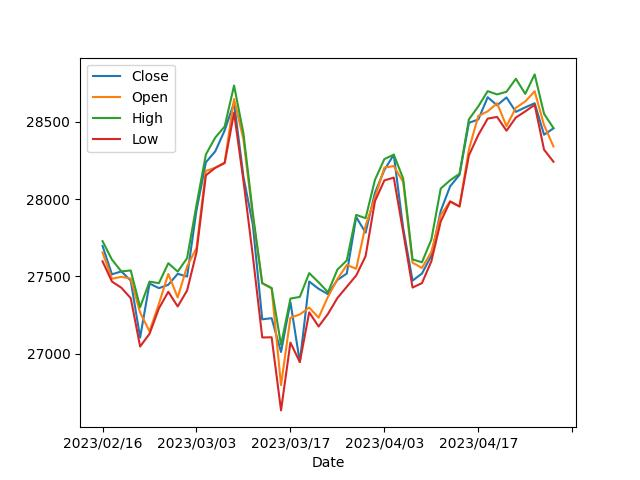
\includegraphics{output3-4.jpeg} \\
    図1 output
\end{center}

\subsection*{工夫した箇所}
株価チャートでよく見るろうそく図を作りたかったがpyplotでは難しいことがわかり断念した。
\\mplfinanceというモジュールを使用したら可能であるというところまでは分かった。今度挑戦しようと思う。
\end{document}